\subsection{线性无关的判定准则}

命题12. 设M是一个投射A-模。对于M中的元素 \(x_1, x_2, \ldots, x_n\) 线性相关，必要且充分条件是存在 \(\lambda \neq 0\) ，以及

\[
\lambda x _ {1} \wedge x _ {2} \wedge \dots \wedge x _ {n} = 0.\tag{22}
\]

该条件是必要的（对 M 不作任何假设），因为例如若 \(\lambda x_{1}\) （其中 \(\lambda \neq 0\) ）是 \(x_{2}, \ldots, x_{n}\) 的线性组合，则关系式 (22) 成立（第 3 号，命题 5）。我们通过对 n 作归纳来证明该条件是充分的；对于 n = 1，它是定义的一个平凡推论。因此假设 n \textgreater{} 1 且条件 (22) 对某个 \(\lambda \neq 0\) 成立。若

\[
\lambda x _ {2} \wedge x _ {3} \wedge \dots \wedge x _ {n} = 0,
\]

成立，则归纳假设蕴含 \(x_{2},\ldots,x_{n}\) 线性相关，从而当然 \(x_{1},x_{2},\ldots,x_{n}\) 也线性相关。若 \(\lambda x_{2}\wedge x_{3}\wedge\cdots\wedge x_{n}\neq0\) ，则由第 8 号定理 1 的推论 3 可知，存在一个交错的 \((n-1)\) -线性形式 f 使得 \(f(\lambda x_{2}\wedge x_{3}\wedge\cdots\wedge x_{n})=\mu\neq0\) 。由于

\[
x _ {1} \wedge (\lambda x _ {2}) \wedge \dots \wedge x _ {n} = 0,
\]

由第 8 号定理 1 的推论 3 可知， \(\mu x_{1}\) 是 \(\lambda x_{2}, x_{3}, \ldots, x_{n}\) 的线性组合；因此 \(x_{1}, x_{2}, \ldots, x_{n}\) 线性相关。

推论. 设M和N是两个投射A-模，且 \(f:M\to N\) 是一个A-线性映射。若f是单射，则 \(\bigwedge(f):\bigwedge(\mathbf{M})\to\bigwedge(\mathbf{N})\) 是单射。

我们首先在M是自由的假设下证明这一点；设 \((e_{\lambda})_{\lambda \in L}\) 是M的一组基，从而 \((e_{J})_{J \in \mathfrak{F}(L)}\) （公式(18)）是 \(\bigwedge(M)\) 的一组基。假设 \(\bigwedge(f)\) 的核包含一个元素 \(u = \sum_{J} \alpha_{J} e_{J} \neq 0\) 。设K是使得 \(\alpha_{J} \neq 0\) 的有限子集J中极小者，并设H是L的一个与K不相交的有限子集，使得 \(K \cup H\) 包含所有（有限个）使得 \(\alpha_{J} \neq 0\) 的 J ；于是对所有满足 \(J \neq K\) 且 \(\alpha_{J} \neq 0\) 的 J ，按定义我们有 \(J \cap H \neq 0\) ，从而（第 8 号，公式 (20)）

\[
u \wedge e _ {\mathrm{H}} = + \alpha_ {\mathbf {K}} e _ {\mathbf {K} \cup \mathbf {H}}
\]

属于 \(\bigwedge (\mathbf{M})\) 的双边理想，即 \(\bigwedge (f)\) 的核。我们记 \(e_{\mathbf{K} \cup \mathbf{H}} = e_{\lambda_1} \wedge e_{\lambda_2} \wedge \dots \wedge e_{\lambda_n}\) ；于是 \(\alpha_{\mathbf{K}} f(e_{\lambda_1}) \wedge f(e_{\lambda_2}) \wedge \dots \wedge f(e_{\lambda_n}) = 0\) ；根据命题 12，N 中的元素 \(f(e_{\lambda_i})\) ( \(1 \leqslant i \leqslant n\) ) 线性相关。但这与假设 \(f\) 是单射（II，§1，第11号，命题17的推论3）相矛盾。

现在我们考虑一般情形；设 \(\mathbf{M}'\) 是一个A-模，使得 \(\mathbf{M} \oplus \mathbf{M}' = \mathbf{P}\) 是自由的（II，§2，第2号，命题4）。考虑线性映射 \(g: \mathbf{M} \oplus \mathbf{M}' \to \mathbf{N} \oplus \mathbf{M} \oplus \mathbf{M}'\) ，它使得 \(g(x, y) = (f(x), 0, y)\) ，从而有交换图

\pandocbounded{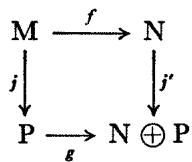
\includegraphics[keepaspectratio]{images/part004_a147f11a.jpg}}

其中竖直箭头是典范单射。由于g是单射且P是自由的， \(\bigwedge(g)\) 如上所见是一个单射同态。现在， \(\bigwedge(j):\bigwedge(\mathbf{M})\to\bigwedge(\mathbf{P})\) 是一个单射同态，因为M是P的一个直因子（第2号）。复合同态

\[
\bigwedge (\mathbf {M}) \xrightarrow {\bigwedge (j)} \bigwedge (\mathbf {P}) \xrightarrow {\bigwedge (g)} \bigwedge (\mathbf {N} \oplus \mathbf {P})
\]

因此是单射的，并且由于它也等于复合同态

\[
\Lambda (\mathbf {M}) \xrightarrow {\Lambda (f)} \Lambda (\mathbf {N}) \xrightarrow {\Lambda (j ^ {\prime})} \Lambda (\mathbf {N} \oplus \mathbf {P})
\]

我们得出结论 \(\bigwedge (f)\) 是单射。

命题13. 设 M 是一个 A-模，N 是 M 的一个直因子子模，它是维数为 p 的自由模，且 \(\{u\}\) 是 \(\bigwedge^{p}(\mathbf{N})\) 的一组基。对于元素 \(x \in M\) 属于 N，必要且充分条件是 \(u \wedge x = 0\) .

设P是M中与N互补的子模，且设 \(y \in N\) , \(z \in P\) 使得 \(x = y + z\) 。则 \(u \wedge x = u \wedge z\) 。由于 \(\bigwedge^{p}(N)\) 是维数为 1 的自由模，映射 \(\phi: P \to P \otimes \bigwedge^{p}(N)\) （它由 \(\phi(p) = p \otimes u\) 给出）是双射（II，§3，第 4 号，命题 4）。另一方面（第7号，命题10），典范同态的复合

\[
\psi : \mathrm{P} \otimes \bigwedge^ {p} (\mathrm{N}) \rightarrow \bigwedge (\mathrm{P}) \otimes \bigwedge (\mathrm{N}) \rightarrow \bigwedge (\mathrm{M})
\]

是单射的。映射 \(\psi \circ \phi\) 因此是单射的，从而命题得证。

定理2. 设 \(\mathbf{M}\) 是一个具有有限基 \((e_i)_{1\leqslant i\leqslant n}\) 的A-模。对于序列 \((x_i)_{1\leqslant i\leqslant n}\) （ \(n\) 个属于 \(\mathbf{M}\) 的元素）构成 \(\mathbf{M}\) 的一个基，必要且充分条件是使得下式成立的元素 \(\lambda \in \mathbf{A}\)

\[
x _ {1} \wedge x _ {2} \wedge \dots \wedge x _ {n} = \lambda . e _ {1} \wedge e _ {2} \wedge \dots \wedge e _ {n}\tag{23}
\]

在 A 中可逆。

请回忆 \(e_{1} \wedge e_{2} \wedge \cdots \wedge e_{n}\) 是 \(\bigwedge^{n}(\mathbf{M})\) 的一个基中的唯一元素（第 8 号，定理 1 的推论 1），因而满足 (23) 的元素 \(\lambda \in A\) 被唯一确定。若 \((x_{i})_{1 \leqslant i \leqslant n}\) 是 M 的一组基，则 \(x_{1} \wedge x_{2} \wedge \cdots \wedge x_{n}\) 是 \(\bigwedge^{n}(\mathbf{M})\) 的一个基中的唯一元素（第 8 号），于是 \(\lambda\) 是可逆的。反之，假设 \(\lambda\) 是可逆的；那么对应于线性映射 \(g: \bigwedge^{n}(\mathbf{M}) \to \mathbf{A}\) （它使得

\[
g (e _ {1} \wedge e _ {2} \wedge \dots \wedge e _ {n}) = \lambda^ {- 1}
\]

）的交错 n-线性形式 f 满足 \(f(x_{1}, x_{2}, \ldots, x_{n}) = 1\) 。对于所有 \(x \in \mathbf{M}\) ，显然

\[
x \wedge x _ {1} \wedge \dots \wedge x _ {n} = 0
\]

（第 3 号，命题 6）；将第 8 号，定理 1 的推论 3 应用于此，我们得到

\[
f (x _ {1}, x _ {2}, \dots , x _ {n}). x = \sum_ {i = 1} (- 1) ^ {i - 1} f (x, x _ {1}, \dots , \hat {x} _ {i}, \dots , x _ {n}). x _ {i}.
\]

由于 \(f(x_{1},\ldots ,x_{n}) = 1\) ，这表明每一个 \(x\in \mathbf{M}\) 都是 \(x_{1},x_{2},\ldots ,x_{n}\) 的线性组合，且由于它们线性无关（因为

\[
x _ {1} \wedge x _ {2} \wedge \dots \wedge x _ {n} \neq 0),
\]

它们构成M的一组基。

